\section{Resultados}

\begin{frame}
	\frametitle{Desalinizador propuesto}
	Se propone un desalinizador de 4 cámaras integradas verticalmente\\
	\begin{figure}
		\centering
		\only<1>{
		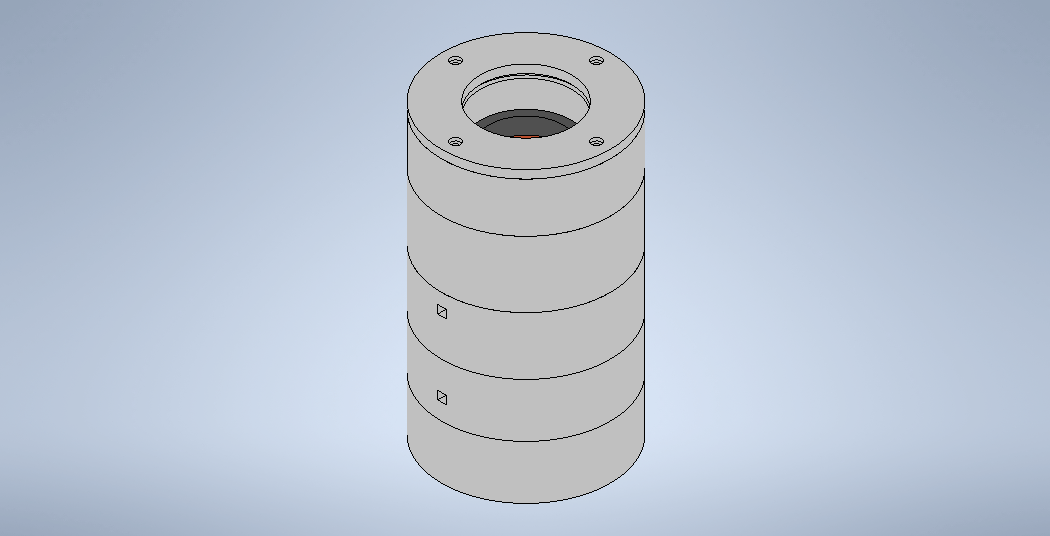
\includegraphics[
			height=60mm,
			width=\linewidth,
			keepaspectratio
		]{Resultados/Sistema/Desalinizador.png}
		}
		\only<2>{
		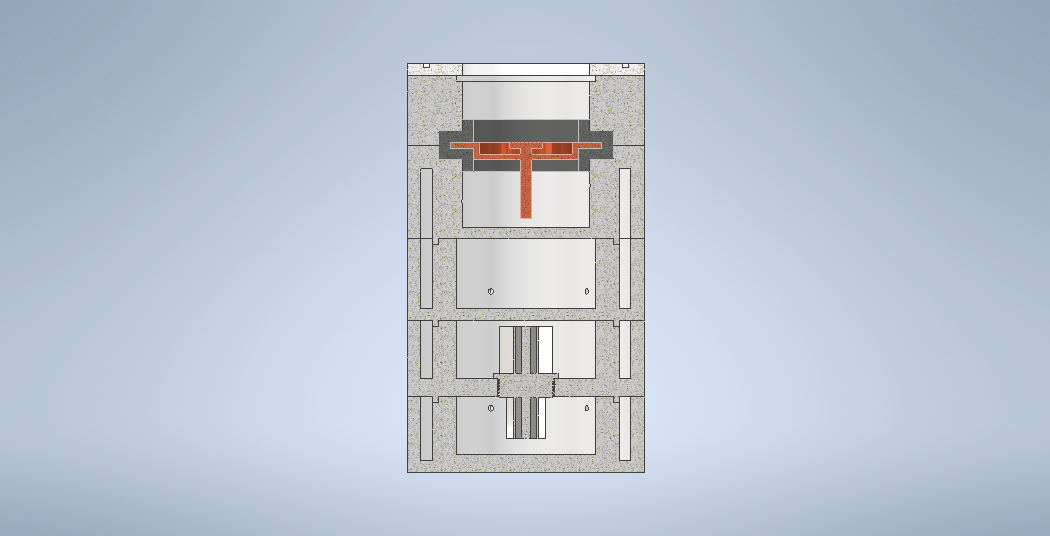
\includegraphics[
			height=60mm,
			width=\linewidth,
			keepaspectratio
		]{Resultados/Sistema/corte-desalinizador.png}
		}
		\caption{Desalinizador propuesto}
	\end{figure}
\end{frame}

\begin{frame}
	\frametitle{Contenedor de agua de mar}
	
	\begin{figure}
		\centering
		\only<1>{
		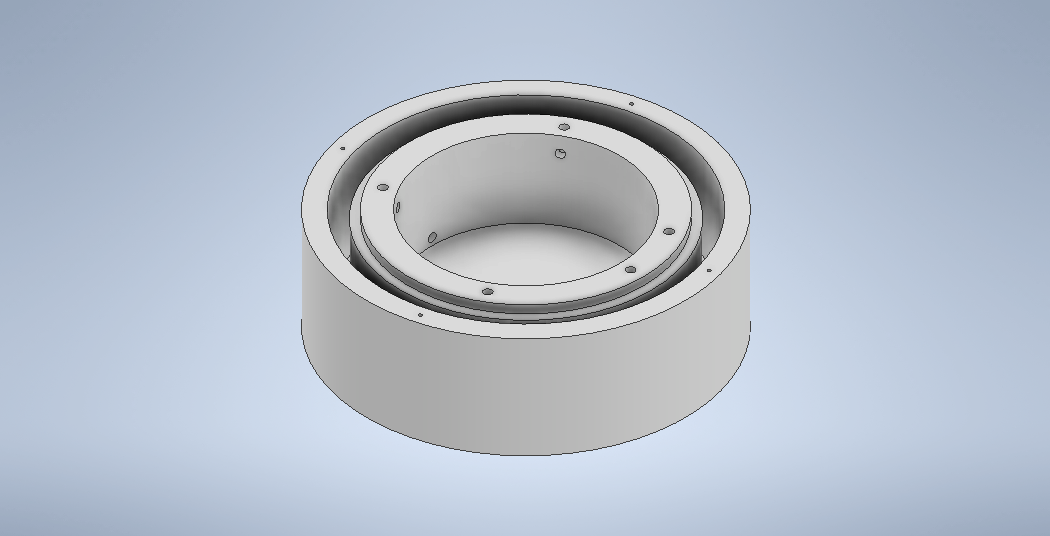
\includegraphics[
			height=45mm,
			width=\linewidth,
			keepaspectratio
		]{Resultados/Cortes/Contenedor-agua-mar.png}
		}
		\only<2>{
		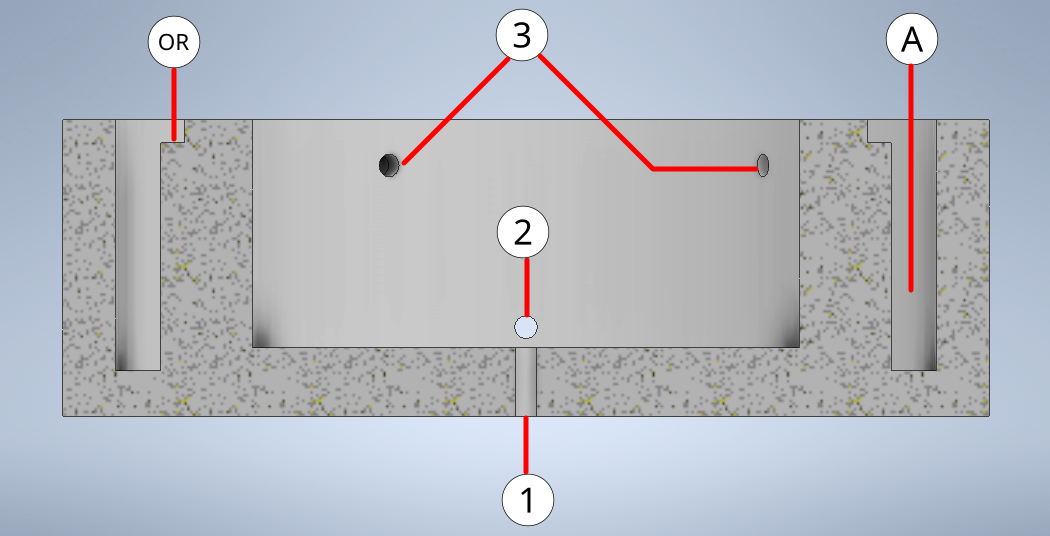
\includegraphics[
			height=45mm,
			width=\linewidth,
			keepaspectratio
		]{Resultados/Cortes/Contenedor-agua-mar-corte-1.png}
		}
		\only<3>{
		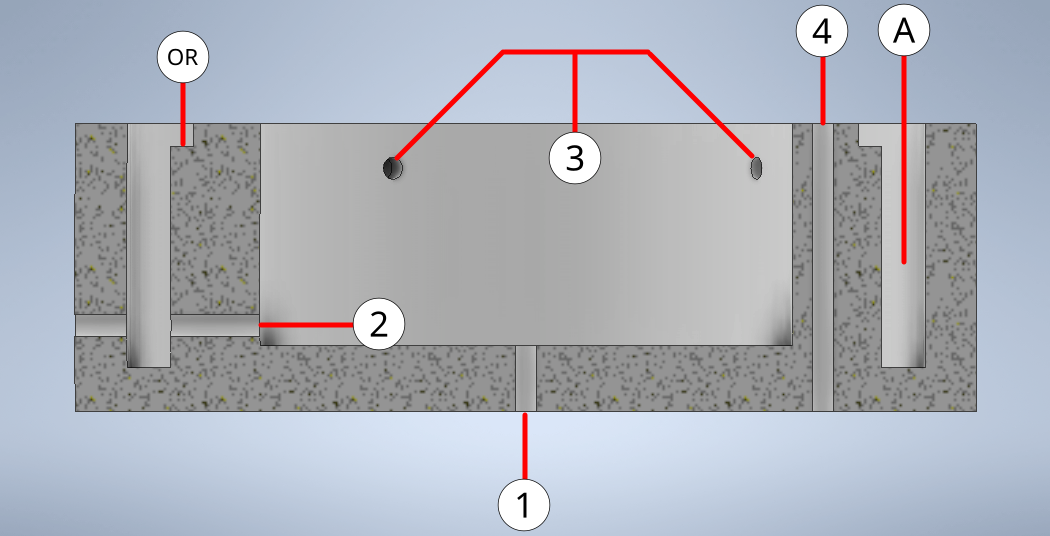
\includegraphics[
			height=45mm,
			width=\linewidth,
			keepaspectratio
		]{Resultados/Cortes/Contenedor-agua-mar-corte-2.png}
		}
		\caption{Contenedor de agua de mar}
	\end{figure}
	
	1) Salida a bomba. 2) Entrada agua. 3) Retroalimentación. 4) Bombeo agua.\\
	OR) Sellado. A) Aislante
	
\end{frame}

\begin{frame}
	\frametitle{Cámara de condensación}
	
	\begin{figure}
		\centering
		\only<1>{
		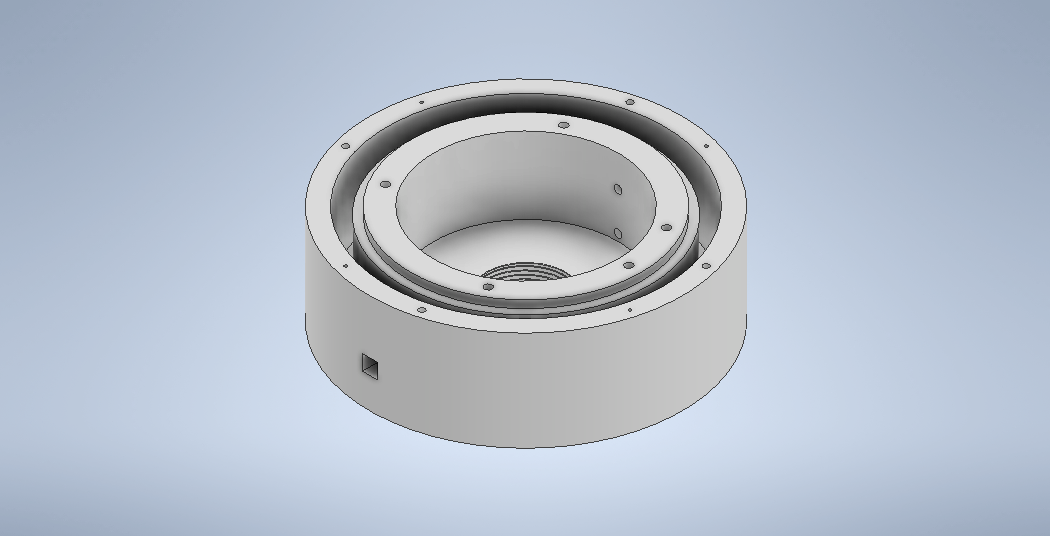
\includegraphics[
			height=45mm,
			width=\linewidth,
			keepaspectratio
		]{Resultados/Cortes/Contenedor-agua-destilada.png}
		}
		\only<2>{
		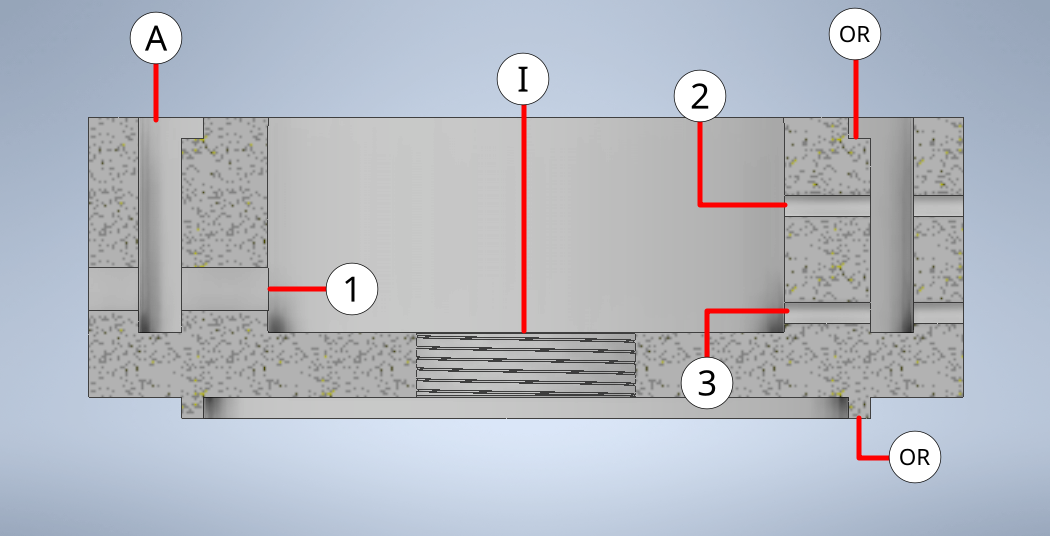
\includegraphics[
			height=45mm,
			width=\linewidth,
			keepaspectratio
		]{Resultados/Cortes/Contenedor-agua-destilada-corte-1.png}
		}
		\only<3>{
		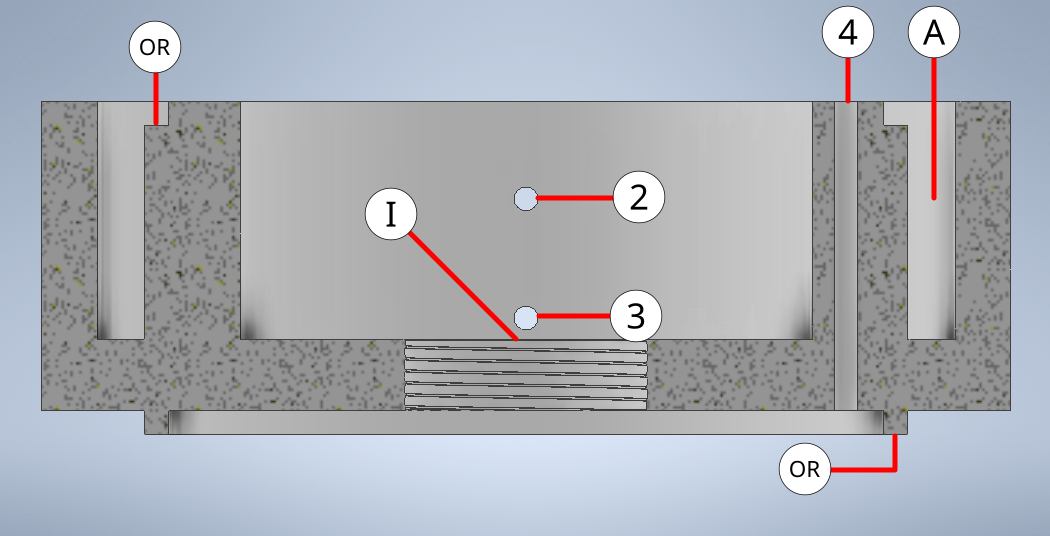
\includegraphics[
			height=45mm,
			width=\linewidth,
			keepaspectratio
		]{Resultados/Cortes/Contenedor-agua-destilada-corte-2.png}
		}
		\caption{Cámara de condensación}
	\end{figure}
	
	1) Entrada vapor. 2) Salida salmuera. 3) Salida agua destilada. 4) Bombeo agua.\\
	
	OR) Sellado. A) Aislante. I) Intercambiador
	
\end{frame}

\begin{frame}
	\frametitle{Intercambiador de calor}
	
	\begin{figure}
		\centering
		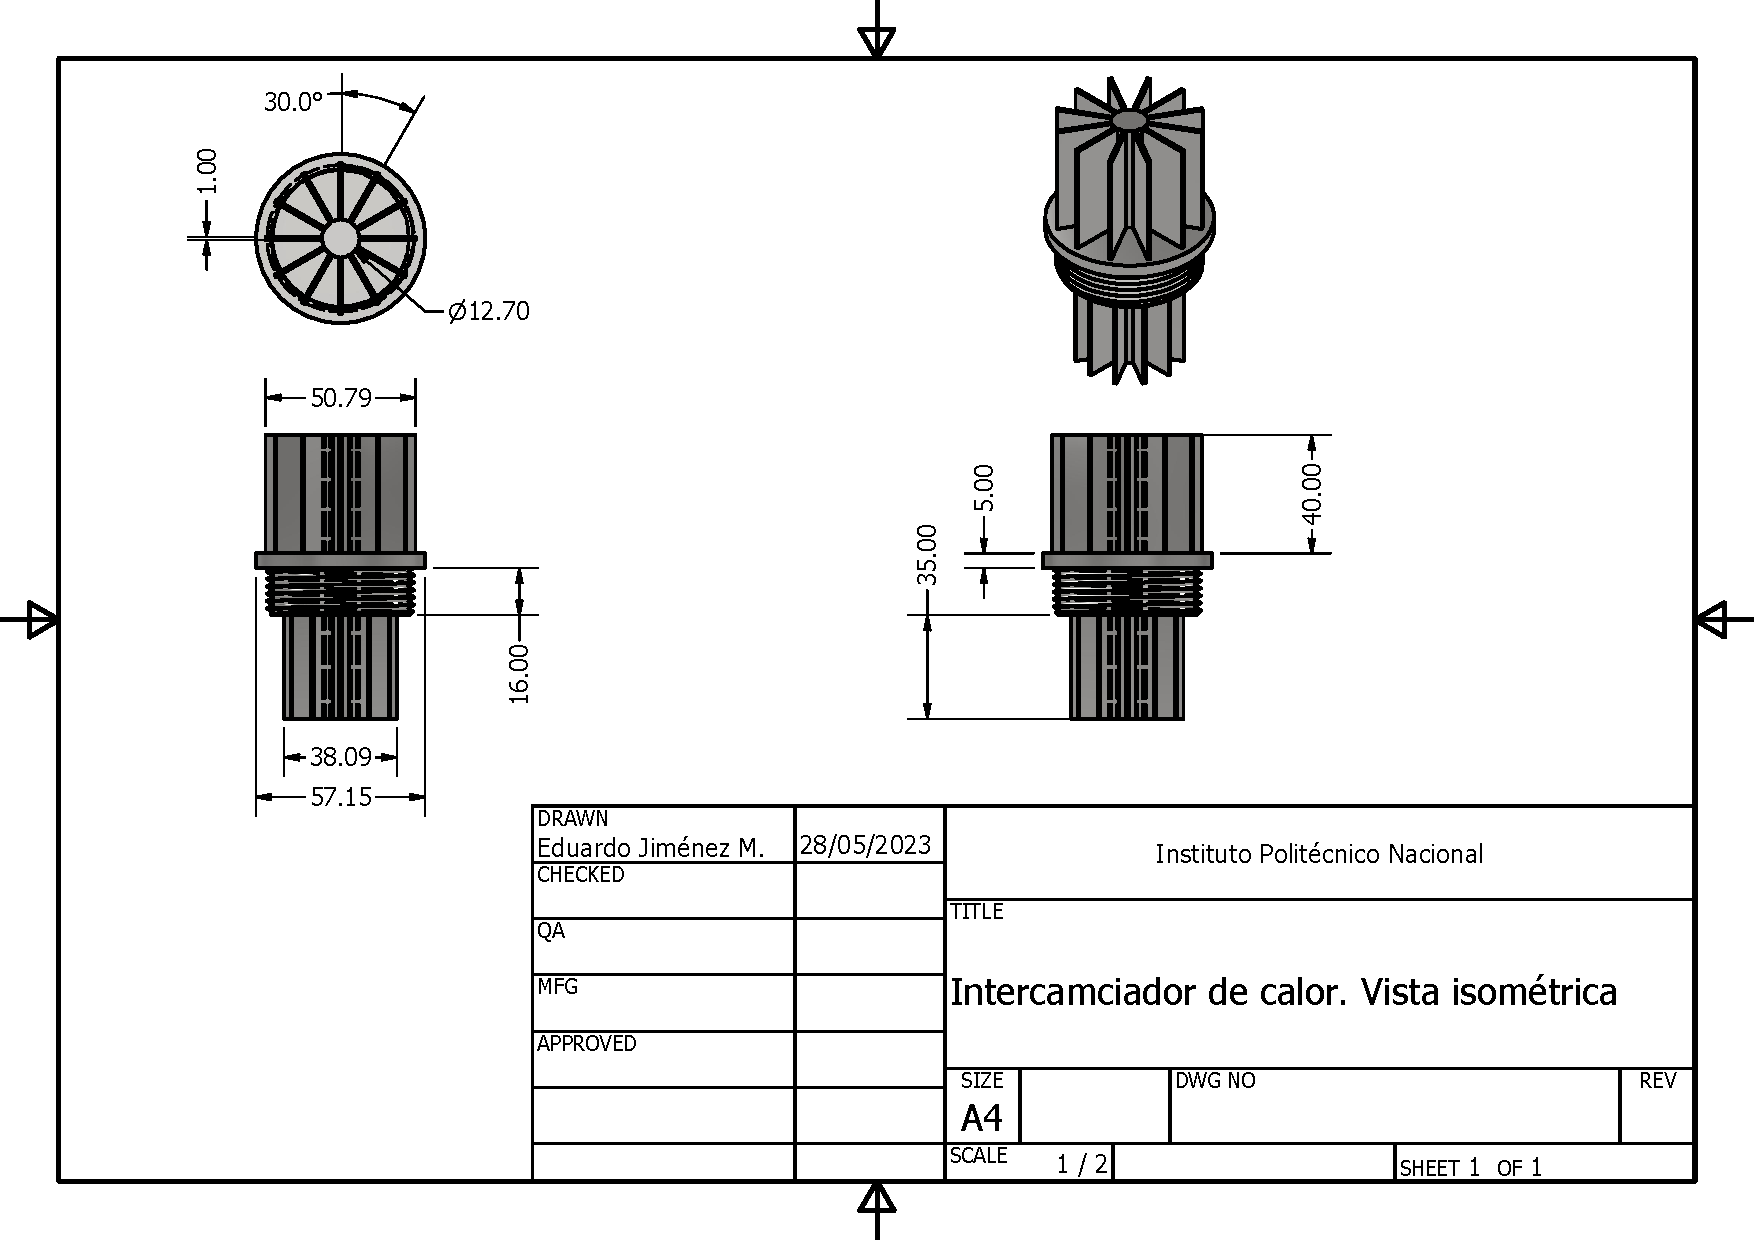
\includegraphics[
			height=75mm,
			width=\linewidth,
			keepaspectratio
		]{Resultados/Sistema/intercambiador.pdf}
		\caption{Intercambiador de acero 316}
	\end{figure}
	
\end{frame}

\begin{frame}
	\frametitle{Cámara de evaporación}
	
	\begin{figure}
		\centering
		\only<1>{
		\includegraphics[
			height=45mm,
			width=\linewidth,
			keepaspectratio
		]{Resultados/Cortes/camara-evaporación.png}
		}
		\only<2>{
		\includegraphics[
			height=45mm,
			width=\linewidth,
			keepaspectratio
		]{Resultados/Cortes/camara-evaporación-corte-1.png}
		}
		\only<3>{
		\includegraphics[
			height=45mm,
			width=\linewidth,
			keepaspectratio
		]{Resultados/Cortes/camara-evaporación-corte-2.png}
		}
		\caption{Cámara de condensación}
	\end{figure}
	
	1) Salida vapor. 2) Salida salmuera. 3) Desagüe. 4) Bombeo agua.\\
	
	OR) Sellado. A) Aislante
	
\end{frame}

\begin{frame}
	\frametitle{Cámara de transferencia parte inferior}
	
	\begin{figure}
		\centering
		\only<1>{
		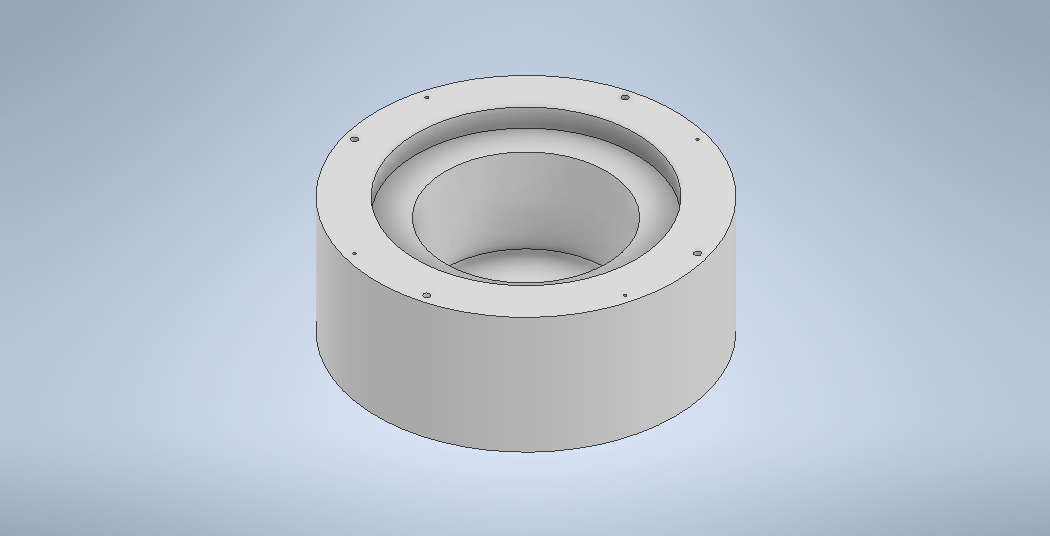
\includegraphics[
			height=45mm,
			width=\linewidth,
			keepaspectratio
		]{Resultados/Cortes/Arena-concentrador.png}
		}
		\only<2>{
		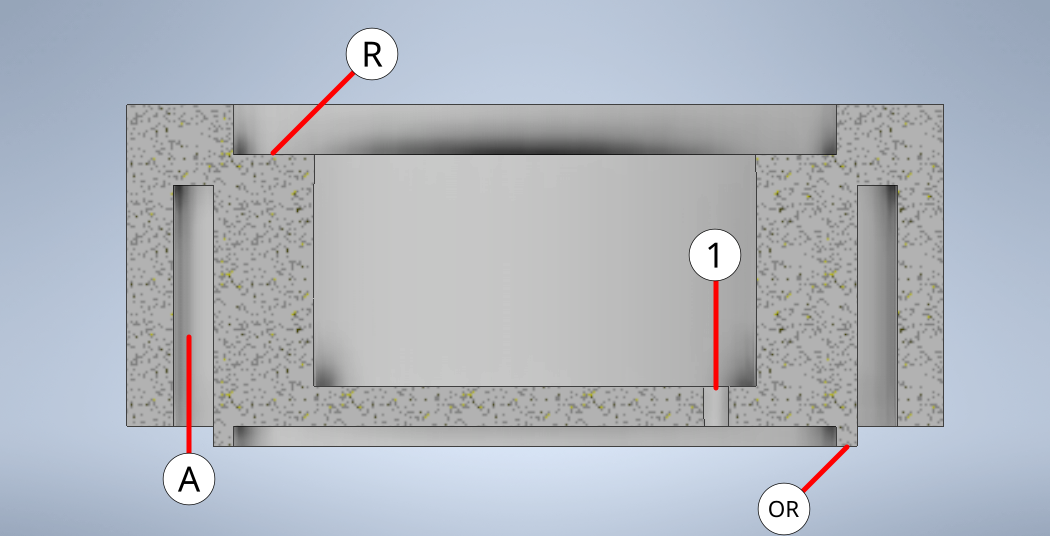
\includegraphics[
			height=45mm,
			width=\linewidth,
			keepaspectratio
		]{Resultados/Cortes/Arena-concentrador-corte-1.png}
		}
		\only<3>{
		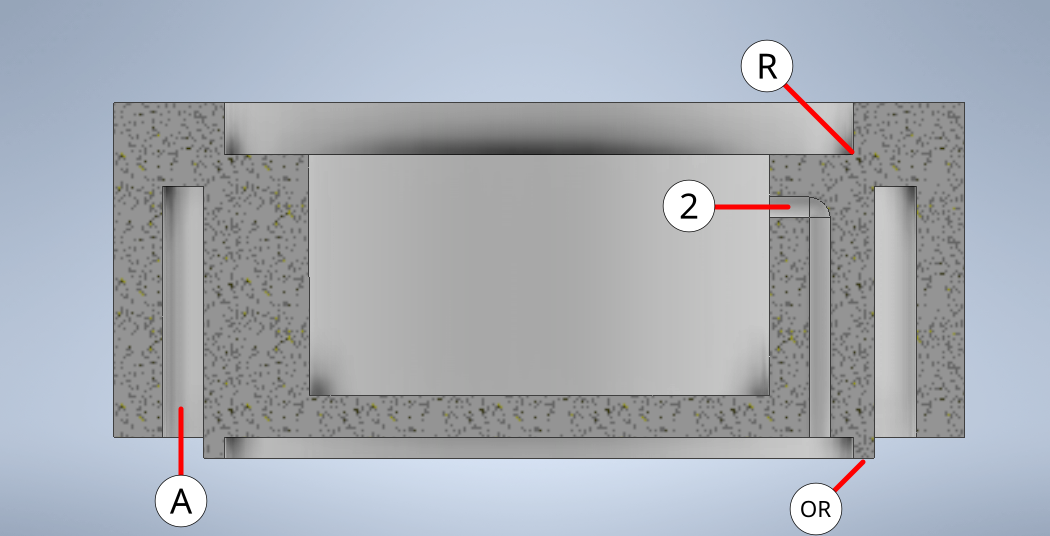
\includegraphics[
			height=45mm,
			width=\linewidth,
			keepaspectratio
		]{Resultados/Cortes/Arena-concentrador-corte-2.png}
		}
		\caption{Cámara de transferencia parte inferior}
	\end{figure}
	
	1) Salida agua caliente. 2) Entrada agua fría \\
	
	OR) Sellado. A) Aislante. R) Recibidor
	
\end{frame}

\begin{frame}
	\frametitle{Cámara de transferencia parte superior}
	
	\begin{figure}
		\centering
		\only<1>{
		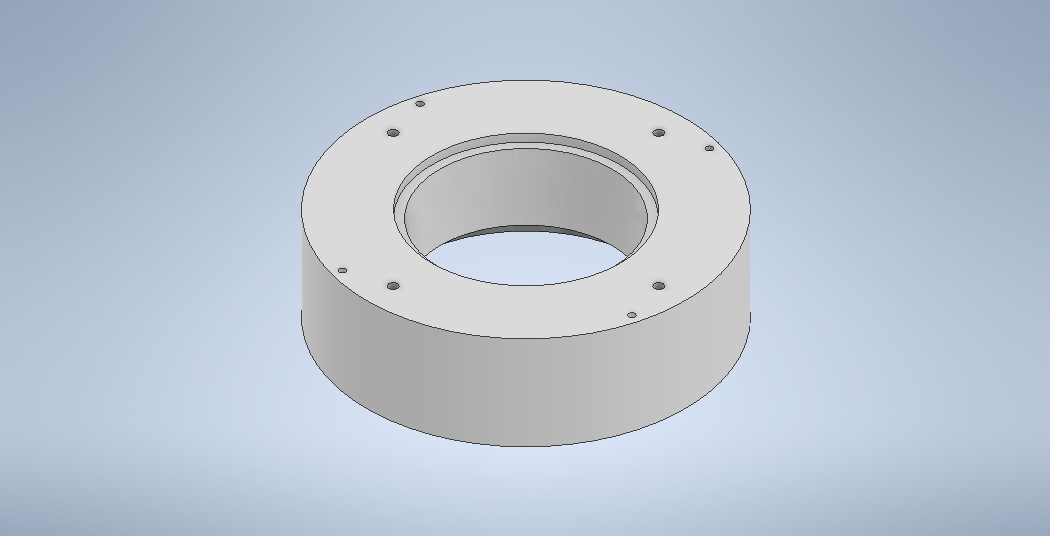
\includegraphics[
			height=45mm,
			width=\linewidth,
			keepaspectratio
		]{Resultados/Cortes/Concentrador.png}
		}
		\only<2>{
		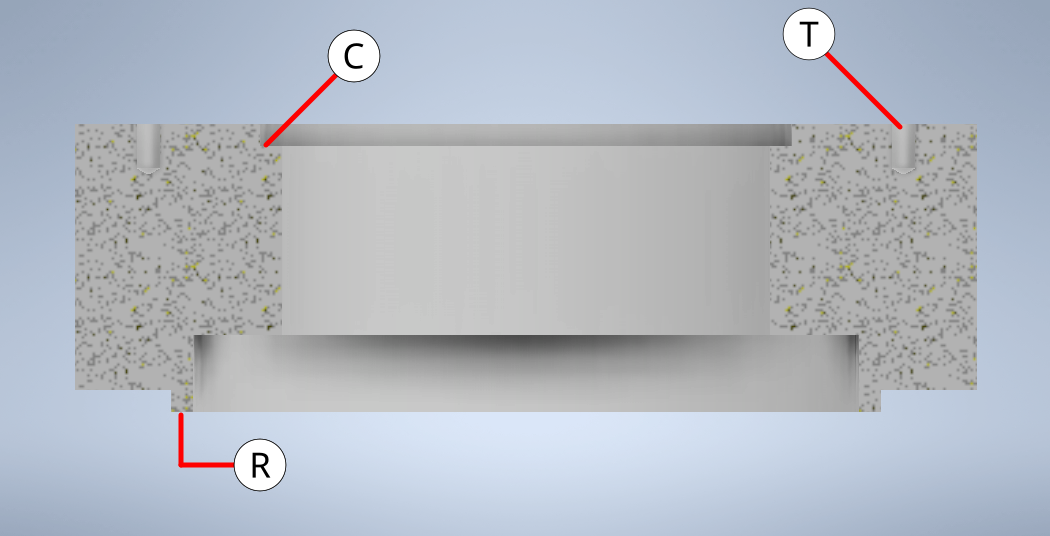
\includegraphics[
			height=45mm,
			width=\linewidth,
			keepaspectratio
		]{Resultados/Cortes/Concentrador-corte-1.png}
		}
		\caption{Cámara de transferencia parte superior}
	\end{figure}
	
	C) Cuarzo. R) Recibidor. T) Tornillo
	
\end{frame}

\begin{frame}
	\frametitle{Recibidor solar}
	
	\begin{figure}
		\centering
		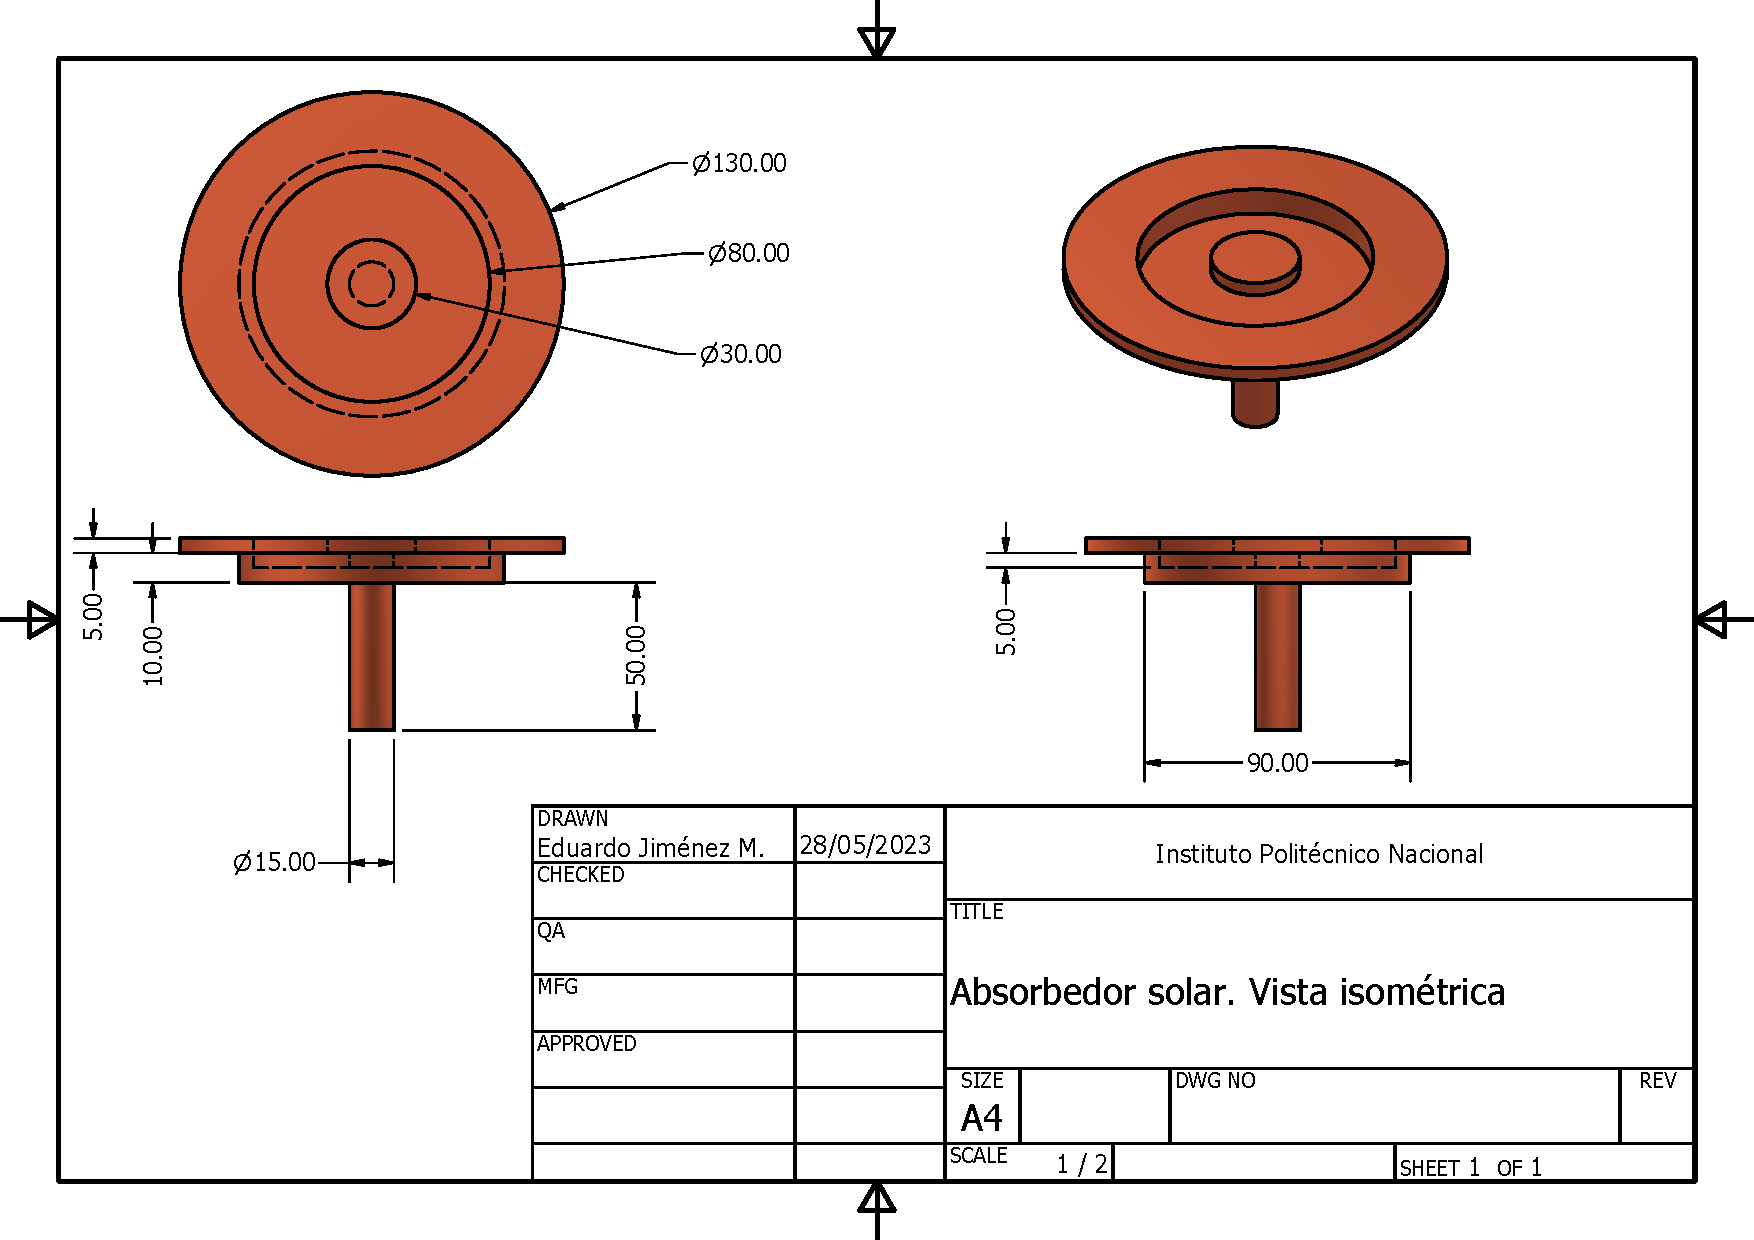
\includegraphics[
			height=70mm,
			width=\linewidth,
			keepaspectratio
		]{Resultados/Sistema/absorbedor.pdf}
		\caption{Recibidor solar}
	\end{figure}
	
\end{frame}